\subsection{Simulation}

A simulation of the Theoretical Development section \ref{DesaTeorico} will be carried out, where the solar panel is modeled with a current source, diodes, and resistors. It will also contain a Buck converter to reduce the voltage, which then passes through a current sensor that will provide the signal to the ESP32 to cut off the current flow to the battery.\\

We will simulate different output voltages from the solar panel to observe how the system behaves. Additionally, each part of the process will be observed.

\begin{figure}[H]
    \centering
    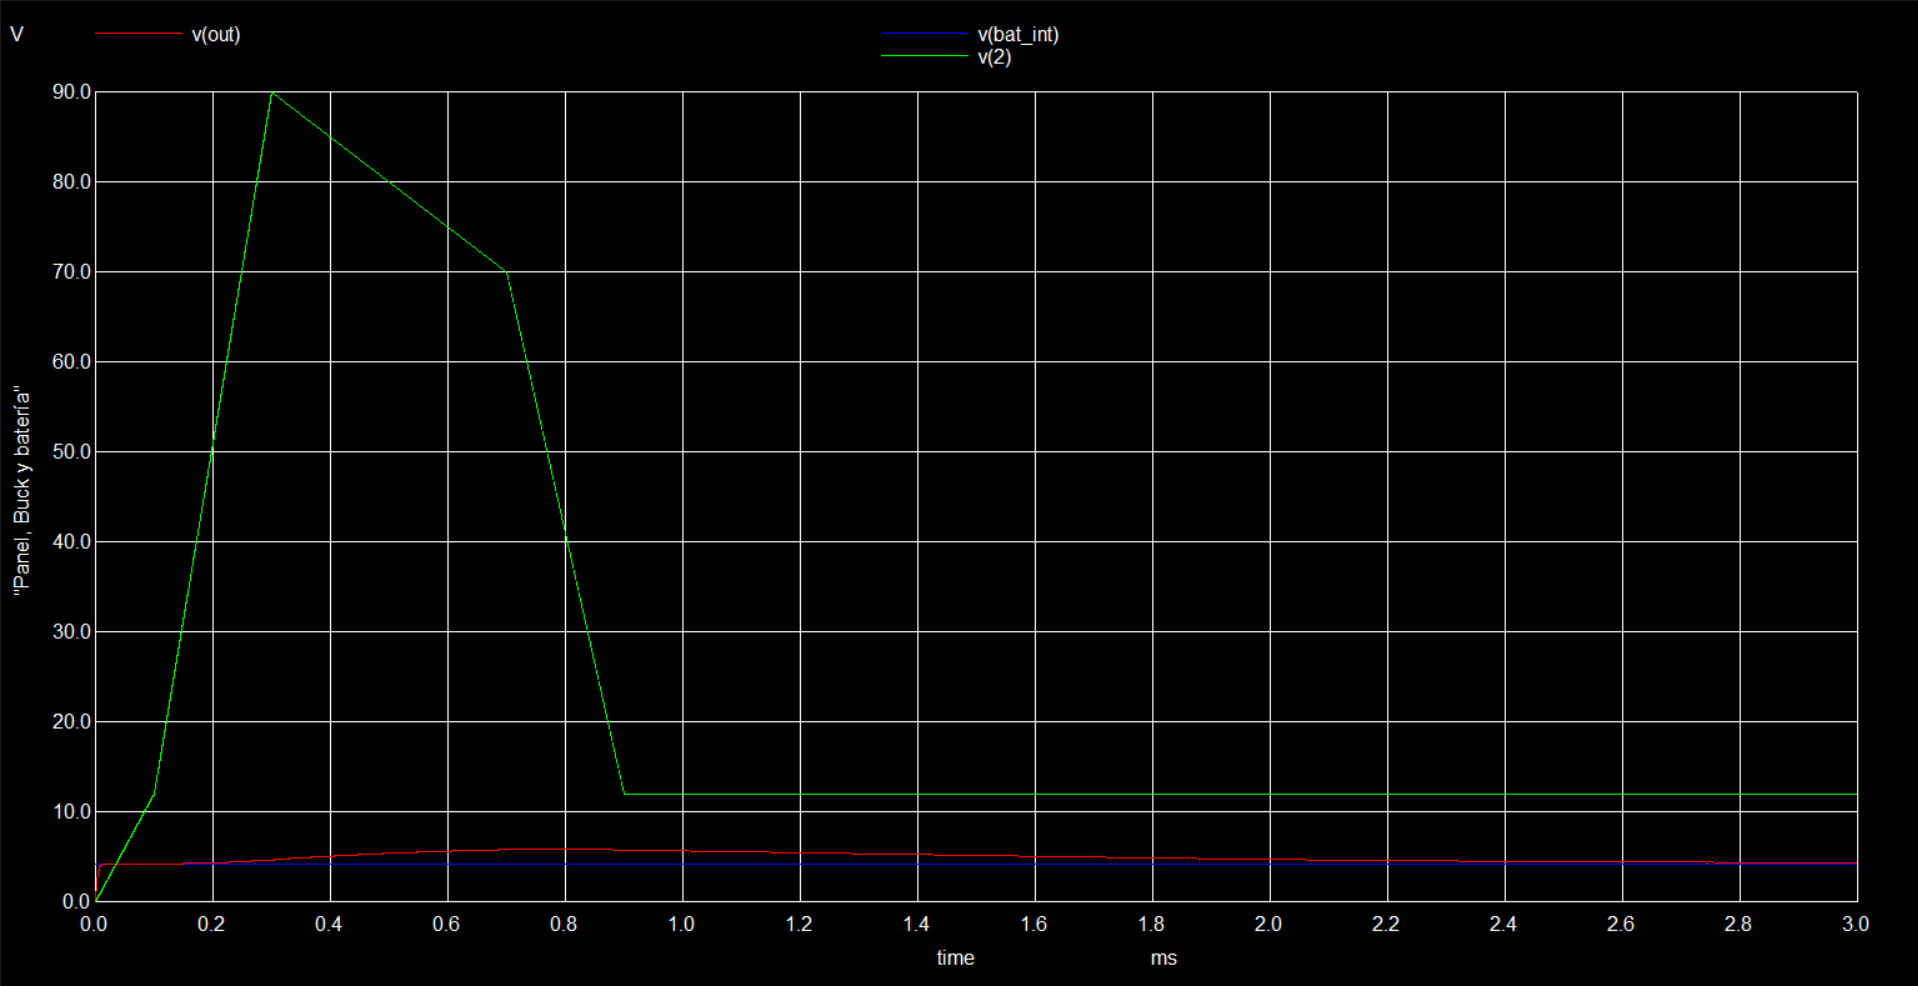
\includegraphics[width=\textwidth]{image/image1}
    \caption{Panel output, converter, and battery status}\label{SIM1}
\end{figure}

In Figure \ref{SIM1}, the voltage changes at the panel's output can be appreciated to see the final behavior. It can be observed that the battery voltage remains constant (possibly due to the short simulation time), while the converter's output tends to stabilize at a value close to $4.20\volt$, where the converter's switch has a frequency of $50\si{\kHz}$ to achieve better regulation of the output voltage.

\begin{figure}[H]
    \centering
    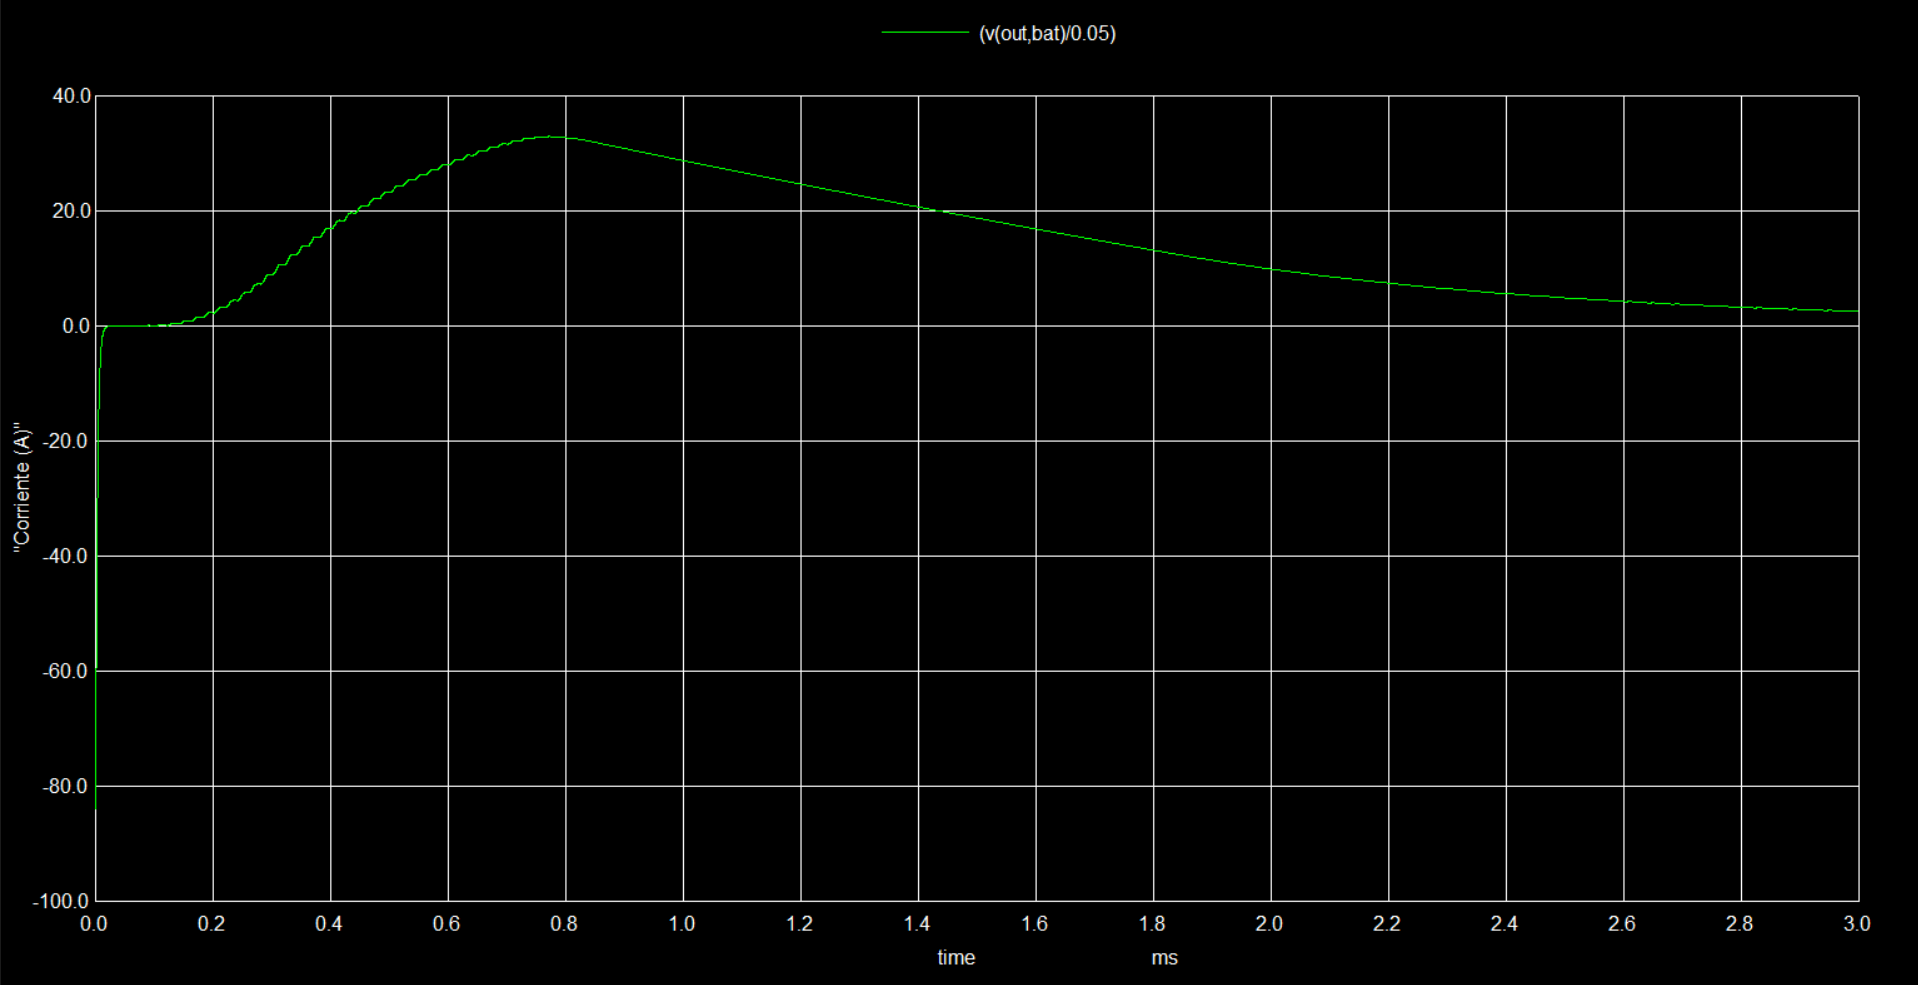
\includegraphics[width=\textwidth]{image/image2}
    \caption{Current Sensor}\label{SIM2}
\end{figure}

In Figure \ref{SIM2}, the current flowing through the shunt resistor for the current sensor can be appreciated. It is observed that it exceeds $5\ampere$ before reaching $400 \si{\micro\second}$, at which point the system should cut off the current flow. Afterwards, with the restoration of the panel voltage, the current decreases again to below $5\ampere$.

\begin{figure}[H]
    \centering
    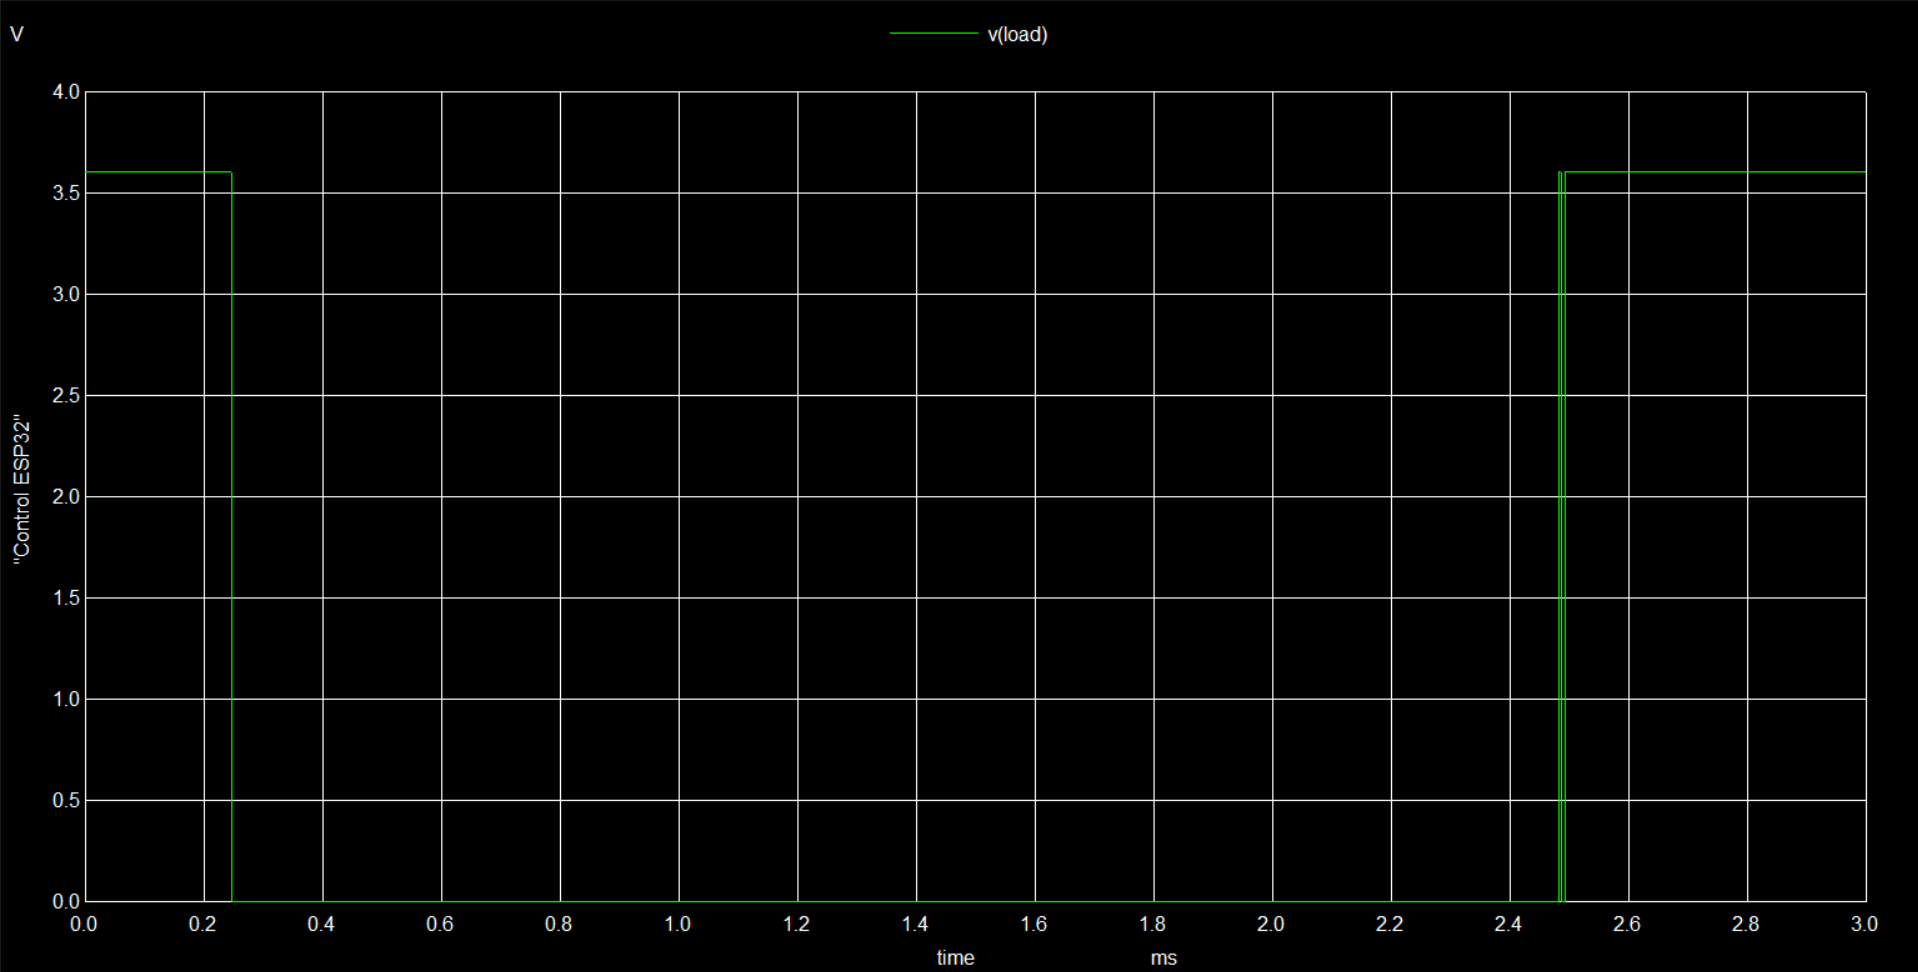
\includegraphics[width=\textwidth]{image/image3}
    \caption{ESP32 Output}\label{SIM3}
\end{figure}

In Figure \ref{SIM3}, it can be observed how the simulation's logic operates: if the Shunt voltage (from the current sensor) is greater than $0.25\volt$, the ESP32 disconnects the system and causes the switch to open. This ensures that no more current flows to the battery. 